
\documentclass[11pt]{article}
\usepackage[paper=letterpaper, margin=.5in]{geometry}
\pdfpagewidth 8.5in
\pdfpageheight 11in
\setlength\parindent{0in}

%% AMS PACKAGES - Chances are you will want some or all of these if writing a math dissertation.
\usepackage{amsmath, amscd, amssymb, amsthm, multirow, enumerate, multicol, graphicx, listings}
\newcommand{\Z}{\mathbb{Z}}
\newcommand{\R}{\mathbb{R}}
\newcommand{\Q}{\mathbb{Q}}
\newcommand{\C}{\mathbb{C}}
\newcommand{\N}{\mathbb{N}}
\newcommand{\V}{\mathbb{V}}
\newcommand{\U}{\mathcal{U}}
\newcommand{\del}{\partial}
\newcommand{\real}{\textrm{Re }}
\newcommand{\imag}{\textrm{Im }}
\newcommand{\pd}[2]{\frac{\partial #1}{\partial #2}}
\newcommand{\deriv}[2]{\frac{d #1}{d #2}}
\newcommand{\sumk}{\sum_{k=1}^\infty}
\newcommand{\sumj}{\sum_{j=1}^\infty}
\newcommand{\sumn}{\sum_{n=0}^\infty}
\newcommand{\summ}[2]{\sum_{k=#1}^{#2}}
\newcommand{\sig}[1]{\sum_{#1 =1}^\infty}
\newcommand{\un}[1]{\bigcup_{#1 =1}^\infty}
\newcommand{\inter}[1]{\bigcap_{#1 =1}^\infty}
\newcommand{\ip}[2]{\langle #1, #2 \rangle}
\newcommand{\ipxu}{\langle x,u_j \rangle}
\newcommand{\uj}{\{u_j\}_{j=1}^\infty}
\newcommand{\B}{\mathcal{B}}

\newcommand{\E}{\mathrm{E}}
\newcommand{\var}{\mathrm{Var}}
\newcommand{\cov}{\mathrm{Cov}}
\newcommand{\ST}{mbox{ s.t. }}

\newcommand{\Example}{\noindent {\bf Example. \quad} }
\newcommand{\Proof}{\noindent {\bf Proof: \quad} }
\newcommand{\Remark}{\noindent {\bf Remark. \quad} }
\newcommand{\Remarks}{\noindent {\bf Remarks. \quad} }
\newcommand{\Case}{\noindent {\underline{Case} \quad} }

\newcommand{\st}{ \; \big | \:}

\newcommand{\deuc}{d_{\mathrm euc}}
\newcommand{\dtaxi}{d_{\mathrm taxi}}
\newcommand{\ddisc}{d_{\mathrm disc}}
\newtheorem{theorem}{Theorem}[section]
\newtheorem{lemma}[theorem]{Lemma}
\newtheorem{proposition}[theorem]{Proposition}
\newtheorem{corollary}[theorem]{Corollary}
\theoremstyle{definition}
\newtheorem{definition}[theorem]{Definition}
\newtheorem{example}[theorem]{Example}

\begin{document}
%%%%%%%%%%%%%%%%%%%%%%%%%%%%%%%%%%%%%%%%%%%%%%%%%%%%%%%%%%%%%%%%%%%%%%%%%%%%%%%%%%%%%%%%%%%%%%%%%%%%%%%%%%%%%%%%%%%%%%%%%%%%%%%%%%%%%
STAT 343, Homework 5 \hfill Aaron Maurer
\vspace{2mm}
\hrule
\vspace{2mm}
\begin{itemize}
    \item[1.]
        \begin{itemize}
            \item[a)] 
                The constant variance assumption apiears to hold; we do not seem to have the variance change over the range of predicted values. The plot on the left, which is the residuals versus the fitted values, indicates by the eyeball test that the distribution of residuals is constant across the range of predicted values. This is shown more formally by the plot on the right, where I have fit a linear model to the square root of the absolute value of each residual in terms of the fitted value. This yields a coefficient of $-.00016$ for the fitted values, with a monstrous p-value of $.969$, dictating that the fitted values of the original regression really don't have any correlation with the deviation of the residuals. \\
                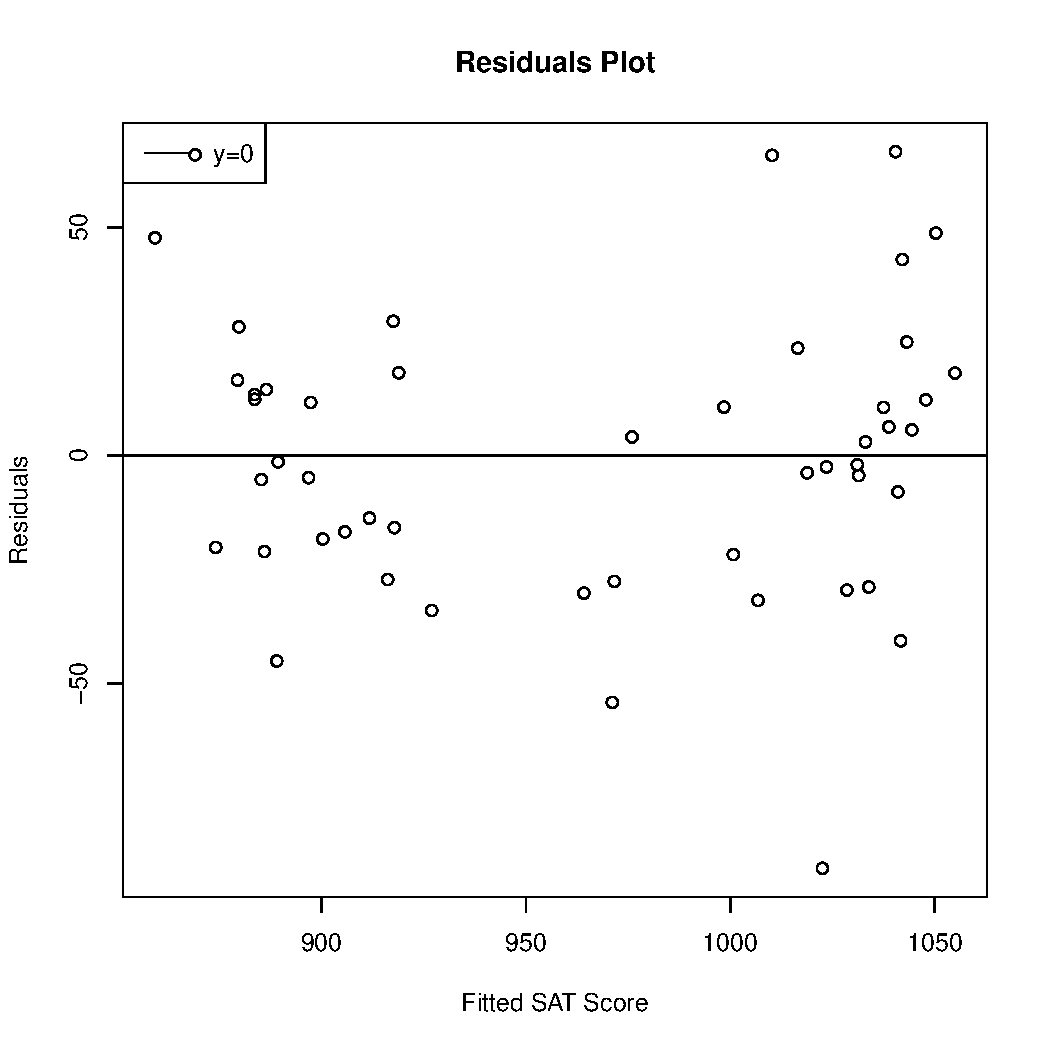
\includegraphics[width=9cm]{hw5_1_a_res} 
                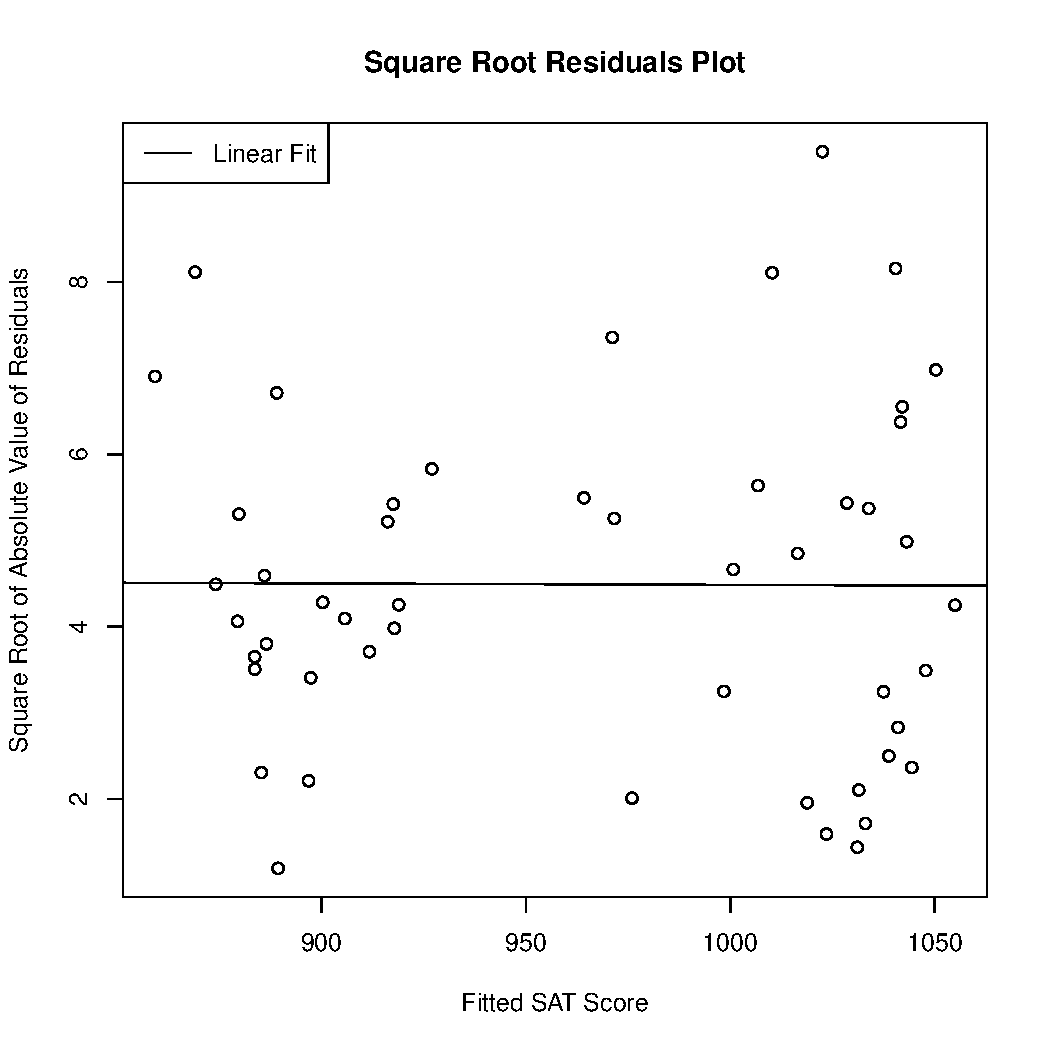
\includegraphics[width=9cm]{hw5_1_a_sqrtres} 
            \item[b)]
                The normality assumption also seems to hold; it appears the residuals are normally distributed around the predicted values. This is indicated by the eyeball test, where we can see from the quantile-quantile plot that the quantiles of the residuals match the quantiles of a normal distribution fairly closely. Additionally, testing that they are normal formally, the Shapiro-Wilkes test yields a p-value of $.430$, which is far to high to reject normality.
                \begin{center}
                    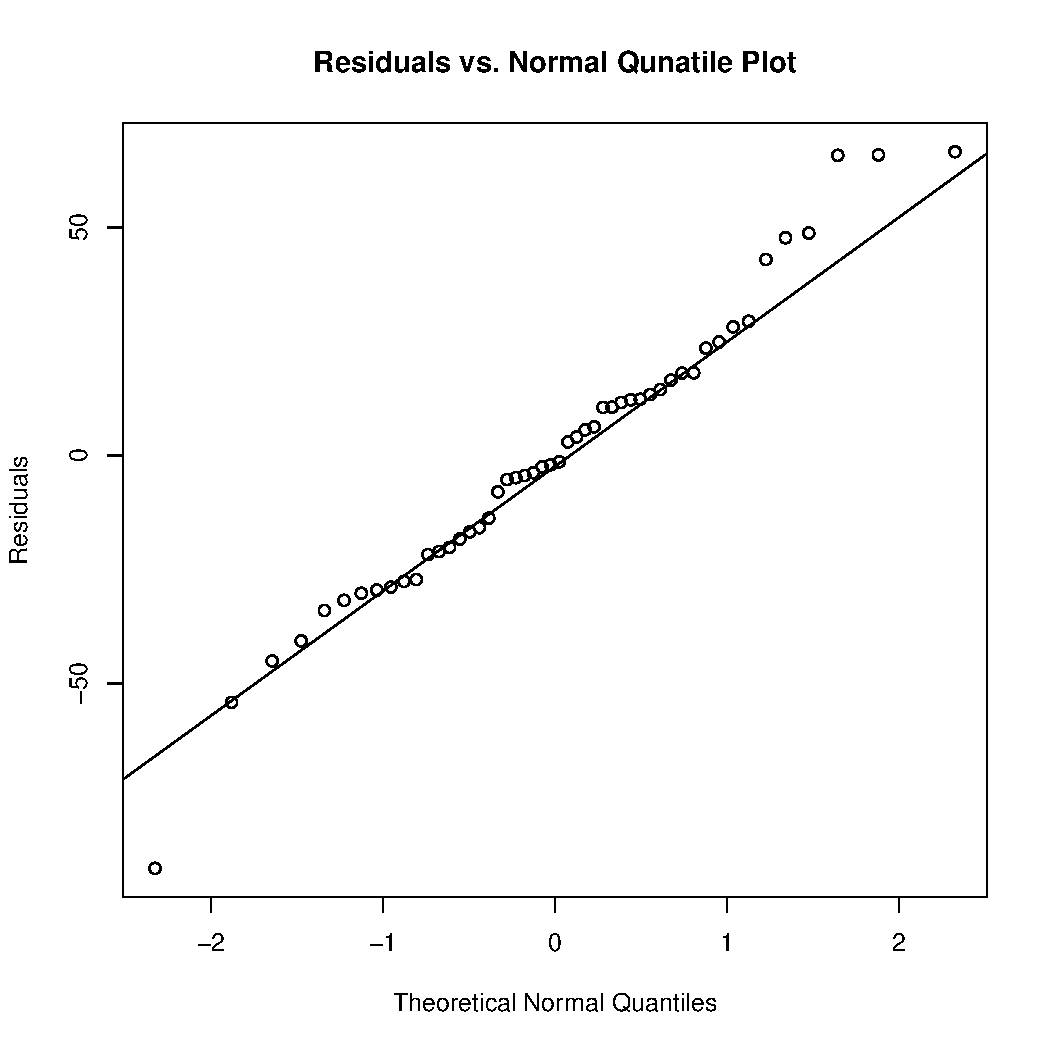
\includegraphics[width=9cm]{hw5_1_b_qq} 
                \end{center}
            \item[c)]
                We do see some points with large leverage, but it doesn't seem that any stand out as being unusually large. I have made a quantile-quantile plot of the leverages against the half normal distribution. We see the states with the highest leverage are Utah followed by California. However, they don't appear to be particular extreme or out of line with the other leverages.
                \begin{center}
                    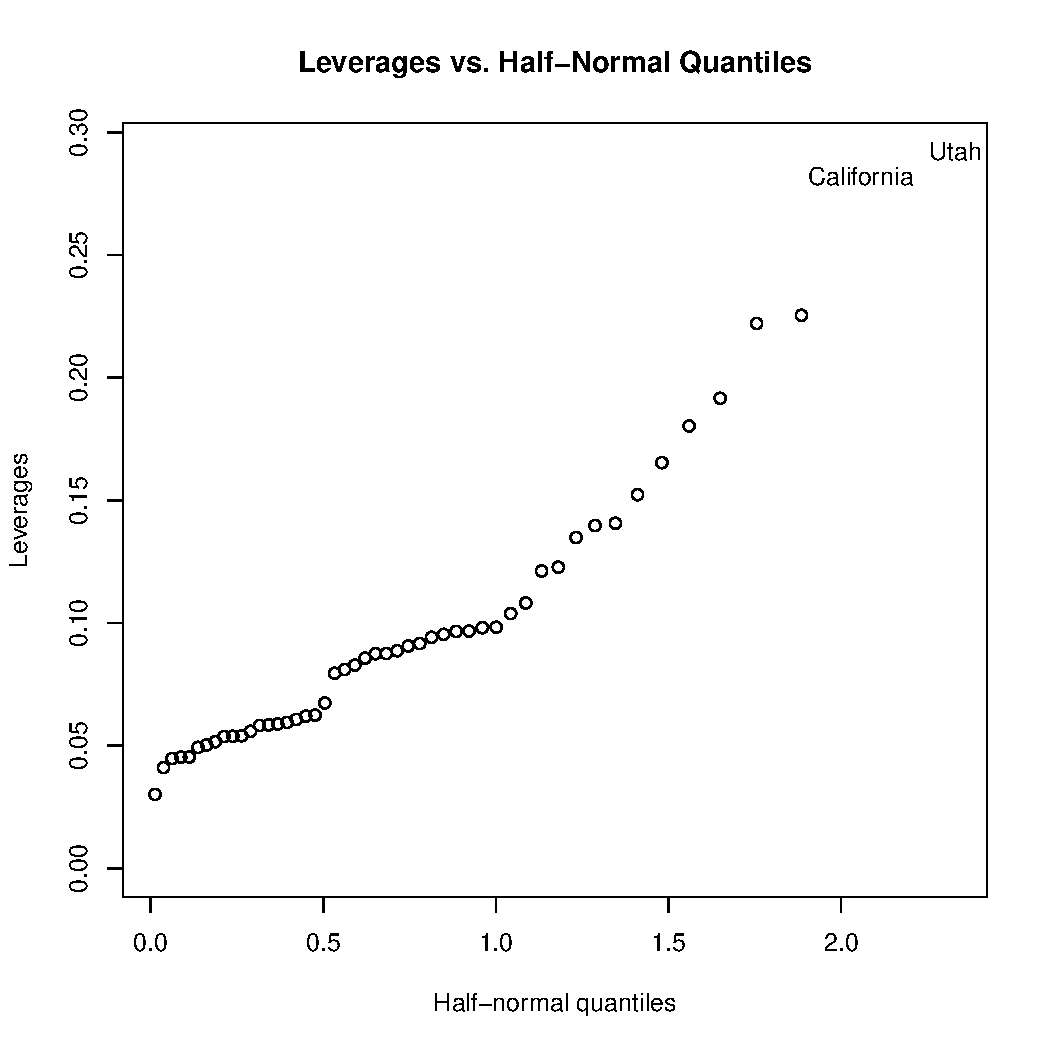
\includegraphics[width=9cm]{hw5_1_c_halfnorm} 
                \end{center}
            \item[d)]
                It doesn't seem that we he have any outliers. The studentized residuals should have a $t_{n-p-1}$ distribution should the assumptions hold, and as we can see from the quantile-quantile plot, that seems to be true. Further, if we look at the most extreme studentized residual, which is the best candidate to be an outlier, we find it is only $-3.124$, which is less than the Bonferroni critical value at a $.1$ alpha level, so we can conclude neither it, nor any other point, is an outlier. 
                \smallskip
                \begin{center}
                    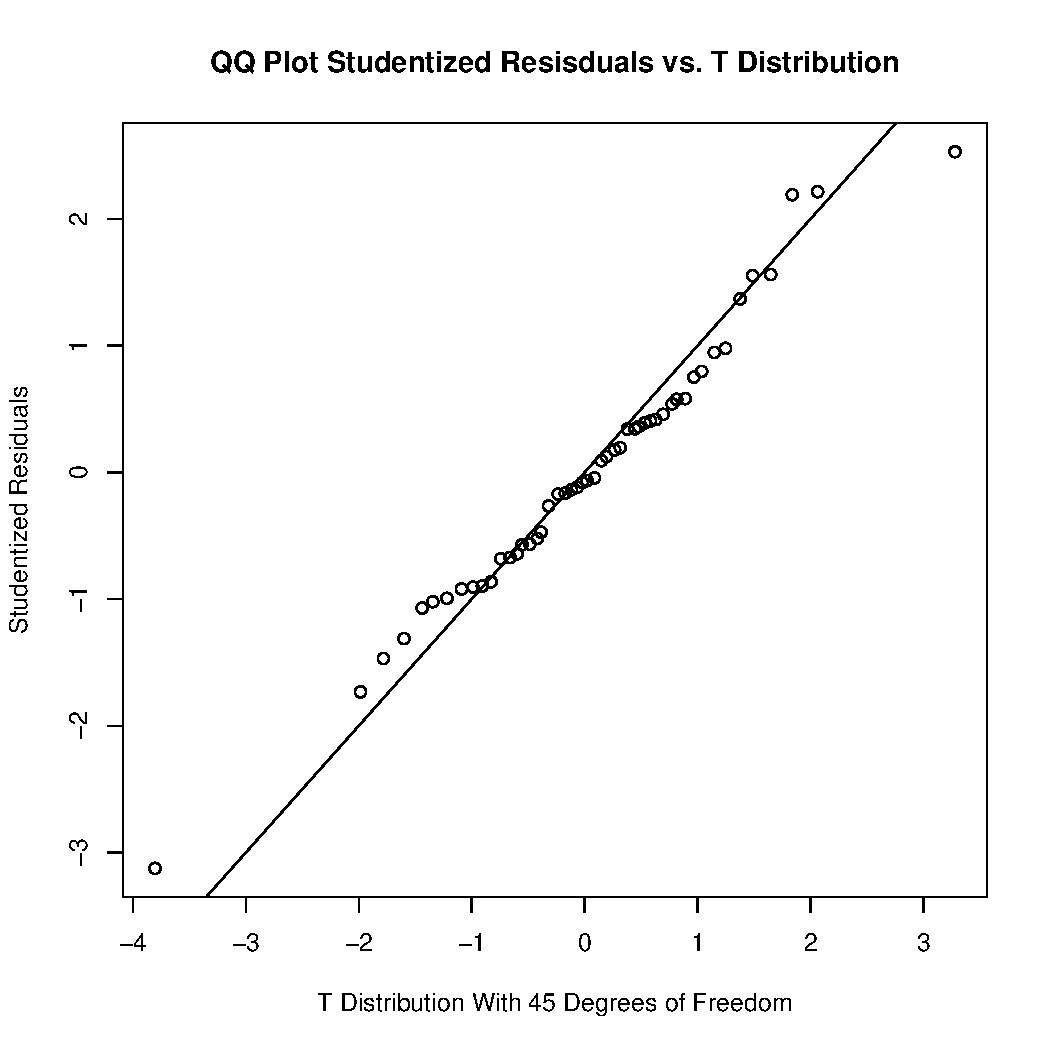
\includegraphics[width=9cm]{hw5_1_d_tqq} 
                \end{center}
                The Bonferroni critical value at an alpha level of $.1$ is the \(\frac{\alpha}{2p}\) quantile of a $t_{n-p-1}$ distribution, giving a value of $-3.281$ in this case. Since the Bonferroni critical value is conservative by construction, I tested at a higher alpha level just to see if their were any outlier candidates.
            \item[e)]
                We seem to have one point that is extremely influential, Utah, and a few additional observations in West Virginia, Florida, New Hampshire and Connecticut which are fairly influential. By looking at the first plot, the Cook Distance, one sees that the inclusion of Utah has far bigger effect on the predictions than any other point, though West Virginia and New Hampshire have pretty large effects in their own right. Looking at the effect of Utah's inclusion on each coefficient individually (the last five graphs), it is the most influential observation on four of the five coefficients, supporting this. However, despite the fact the cook distance of Connecticut and Florida wasn't that high, they are each fairly influential on a few variables. New Hampshire and West Virginia are fairly influential on a variable or two a piece as well, as the cook distance pointed to.
                \begin{center}
                    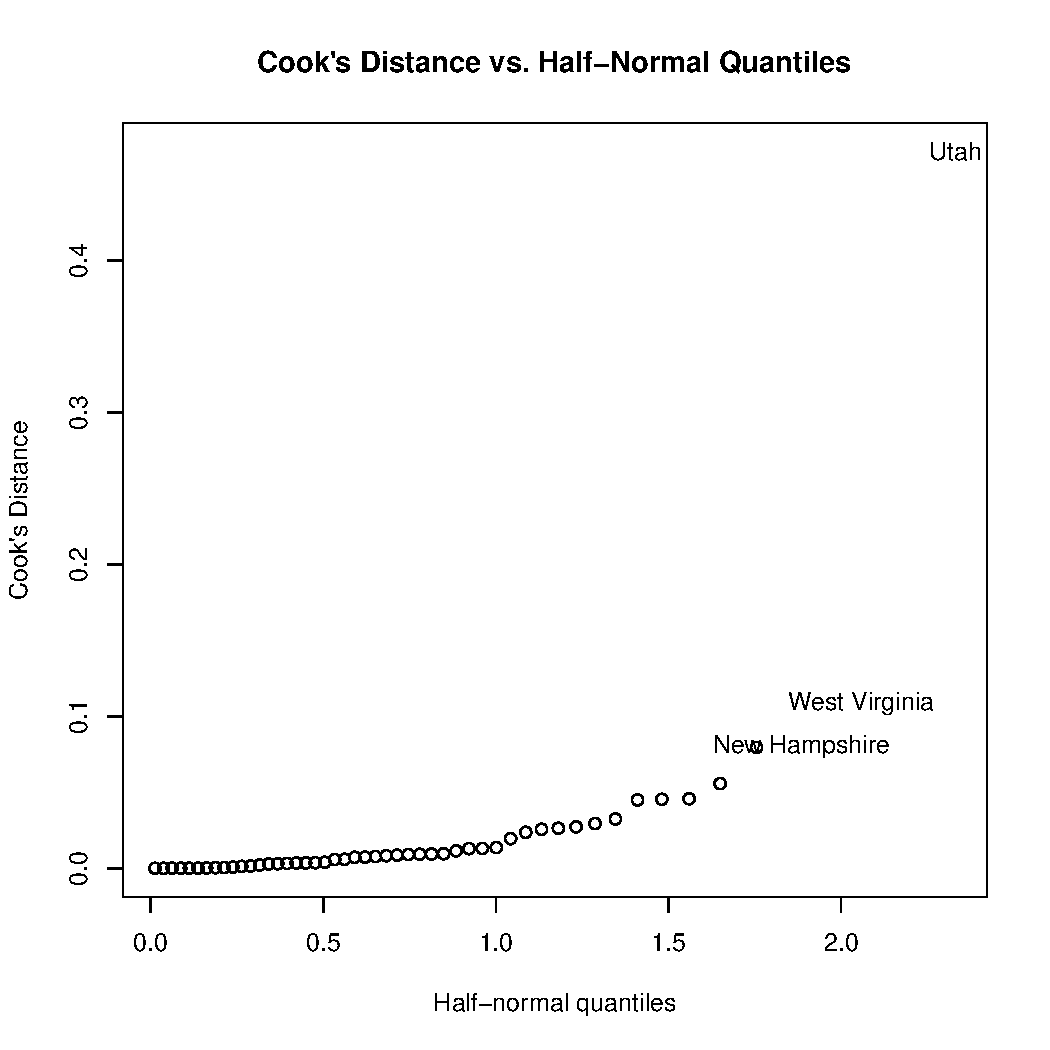
\includegraphics[width=9cm]{hw5_1_e_halfnorm} 
                \end{center}
                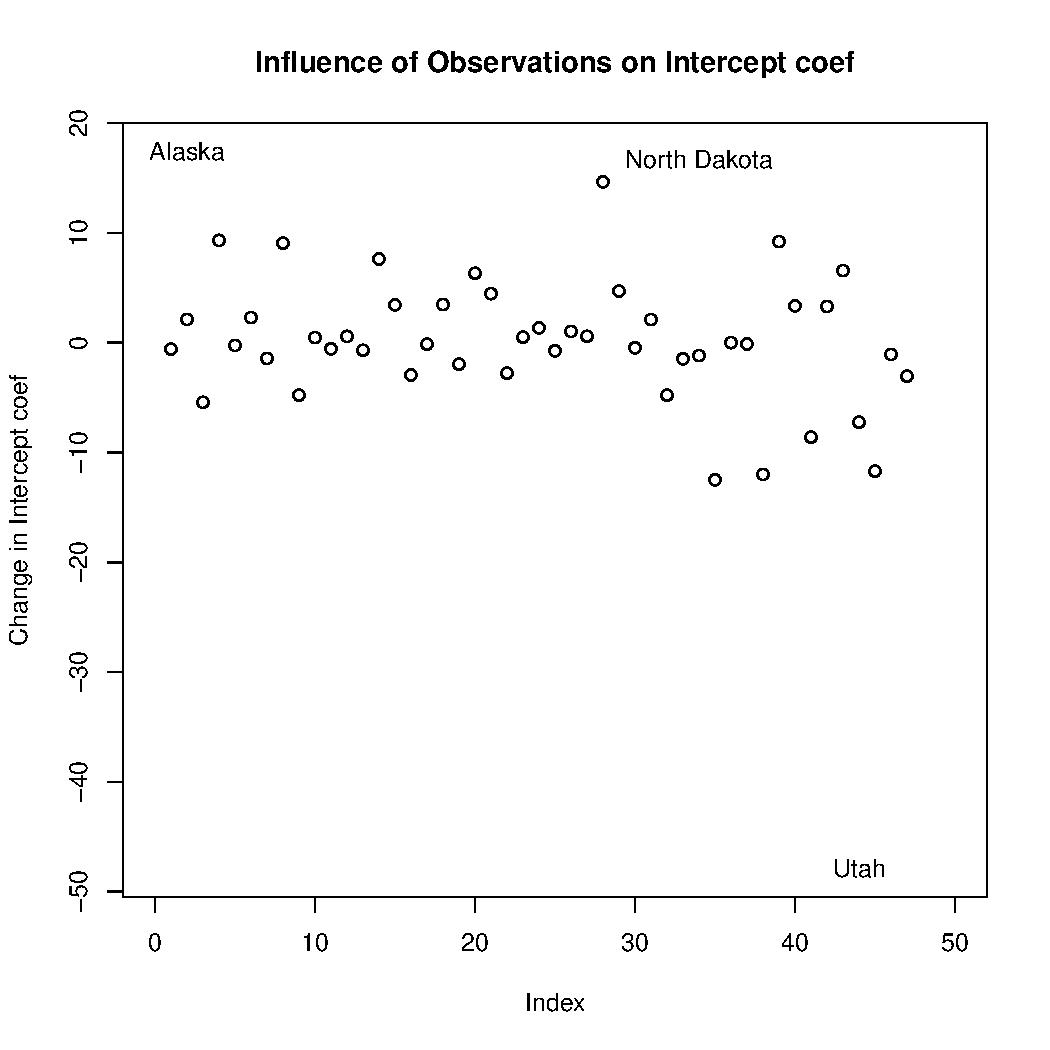
\includegraphics[width=9cm]{hw5_1_e_Intercept}
                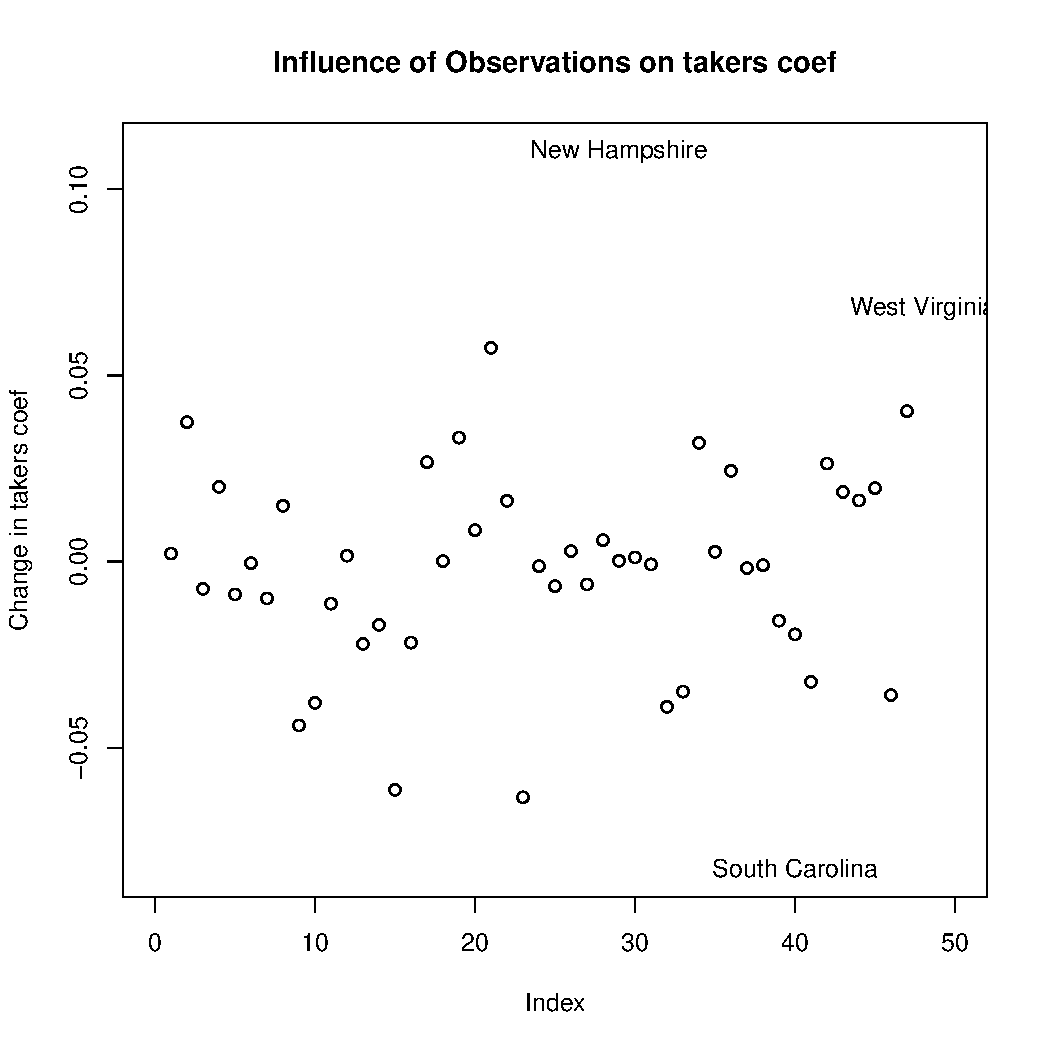
\includegraphics[width=9cm]{hw5_1_e_takers} \\
                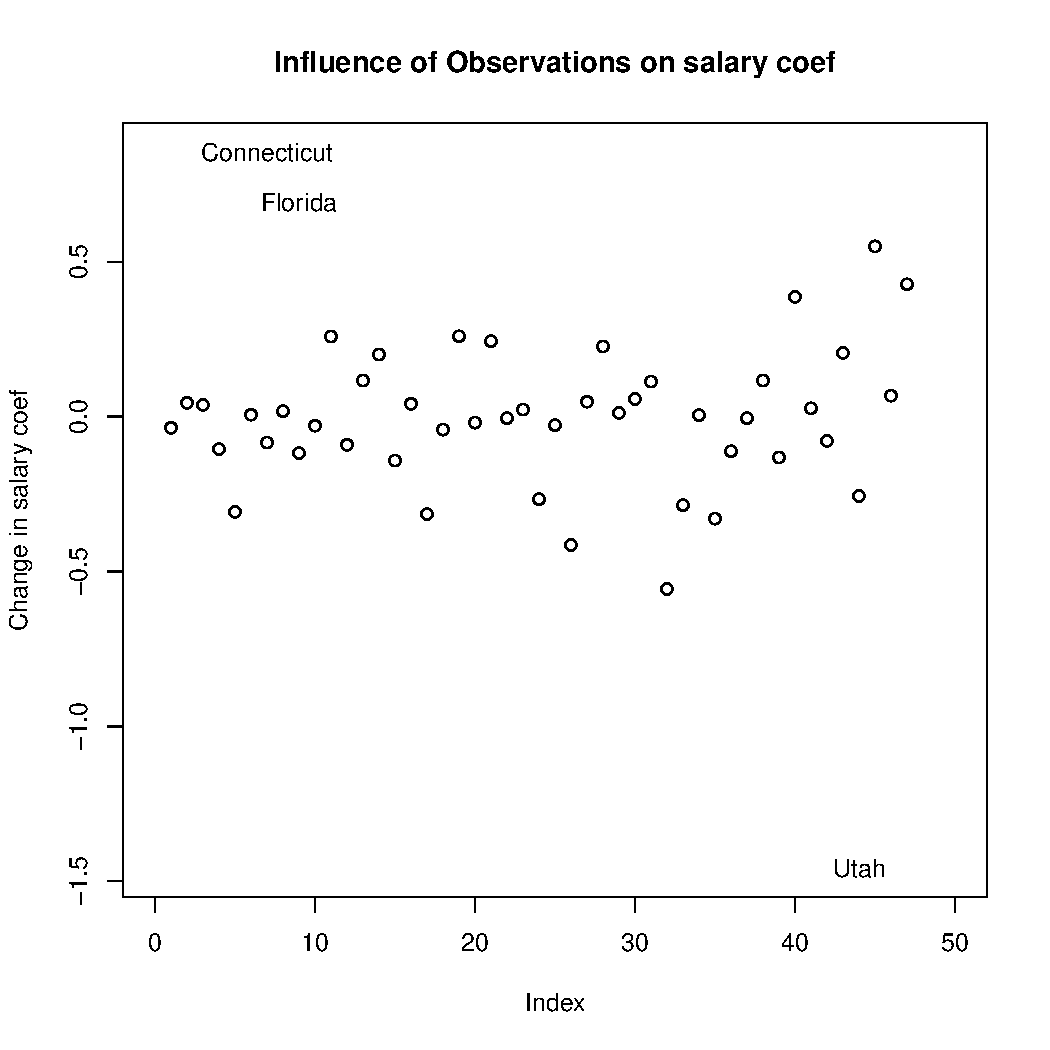
\includegraphics[width=9cm]{hw5_1_e_salary} 
                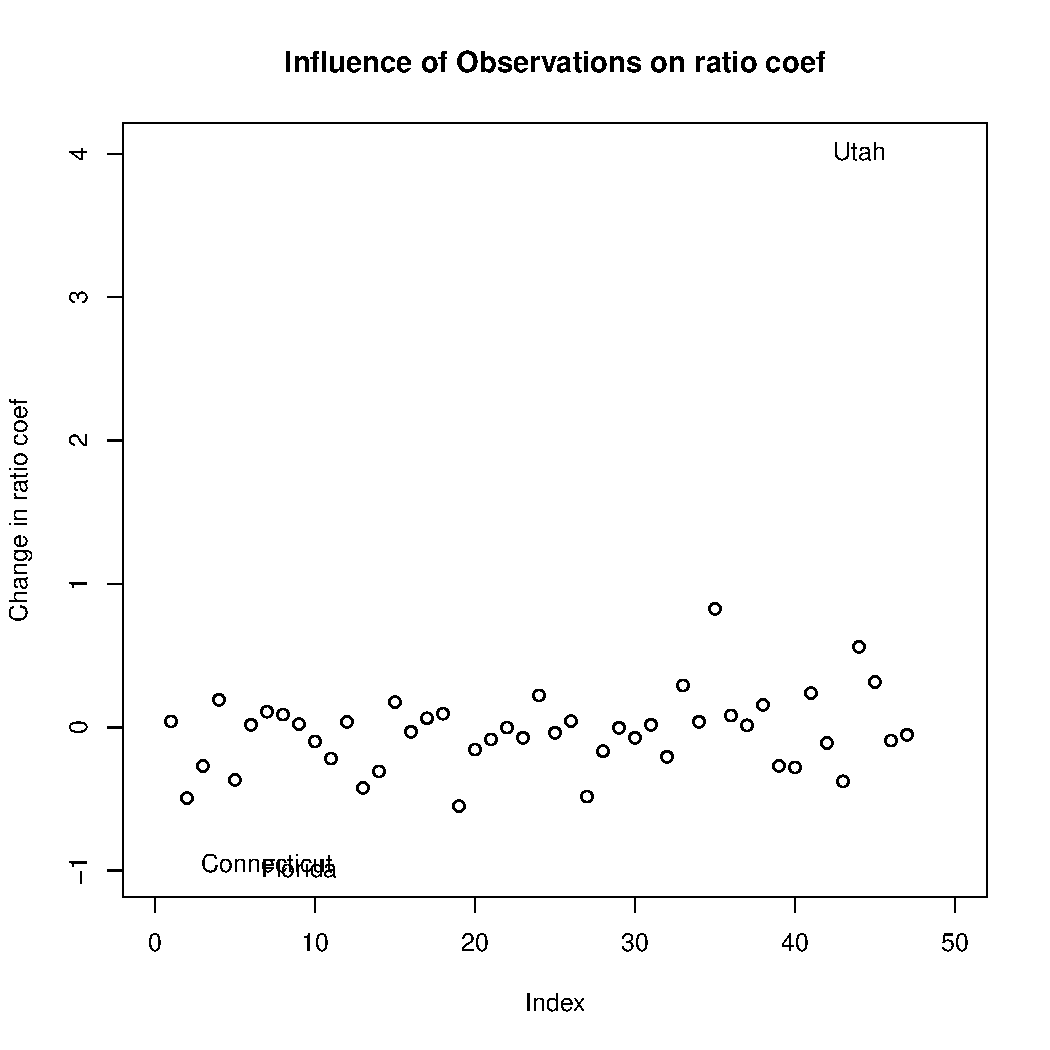
\includegraphics[width=9cm]{hw5_1_e_ratio}  \\
                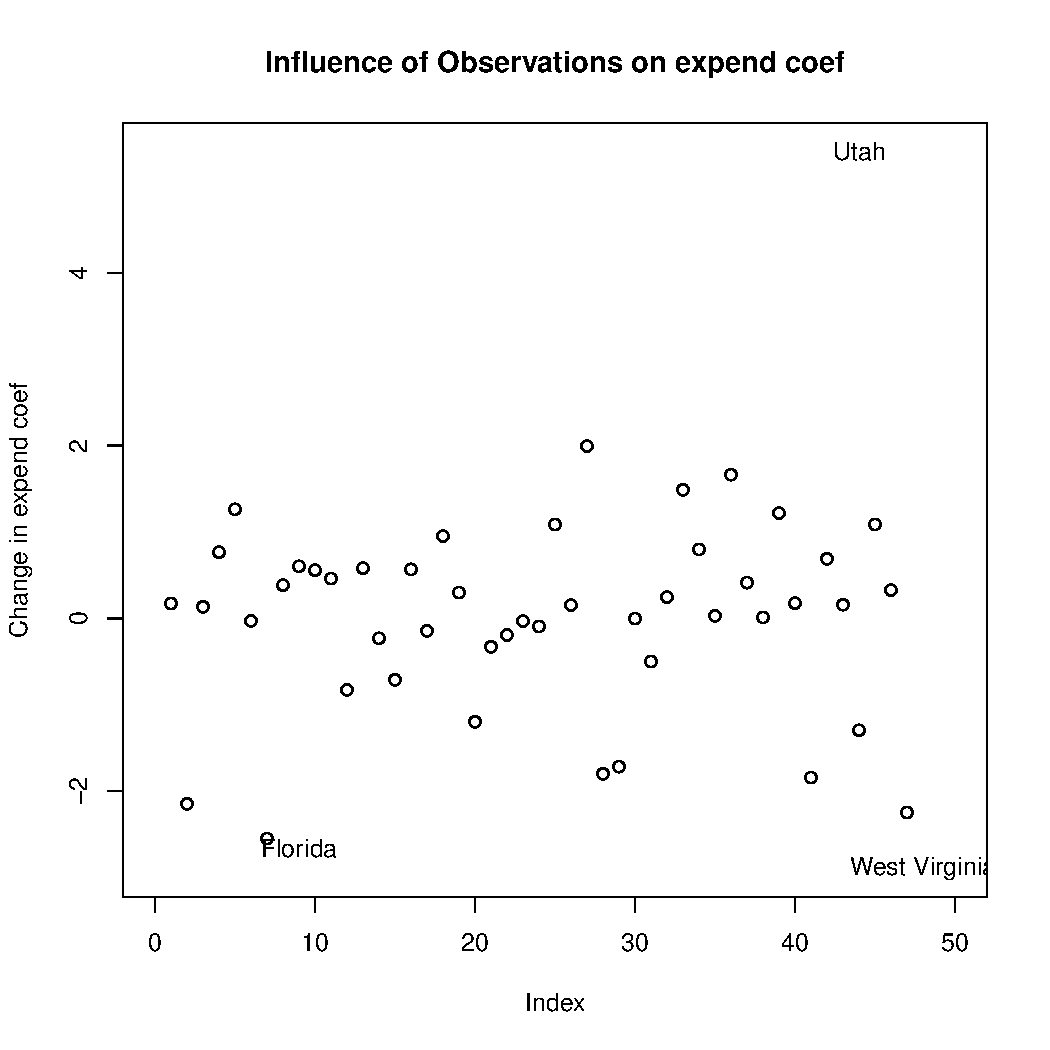
\includegraphics[width=9cm]{hw5_1_e_expend} 
            \item[f)]
                The assumption that there is a linear relationship between the predictors and the outcome does not quite seem to hold. We can see this most clearly when we try to predict the residuals based on the predicted values with a more flexible local linear regression (the first plot); when we do, we can see that the mean of the residuals is lower than $0$ in the center of the predicted values, and higher on the edges, indicating a non-linear, possibly quadratic relationship. Digging into this further, repeating this process on the four partial residual plots (the last four plots), it seems like this is because there is a non-linear fit between takers and the outcome. For the other three variables, while the local linear regressions may be picking up some meaningful non-linearity, they generally appear to just be fluctuating around the linear fit with noise.
                \begin{center}
                    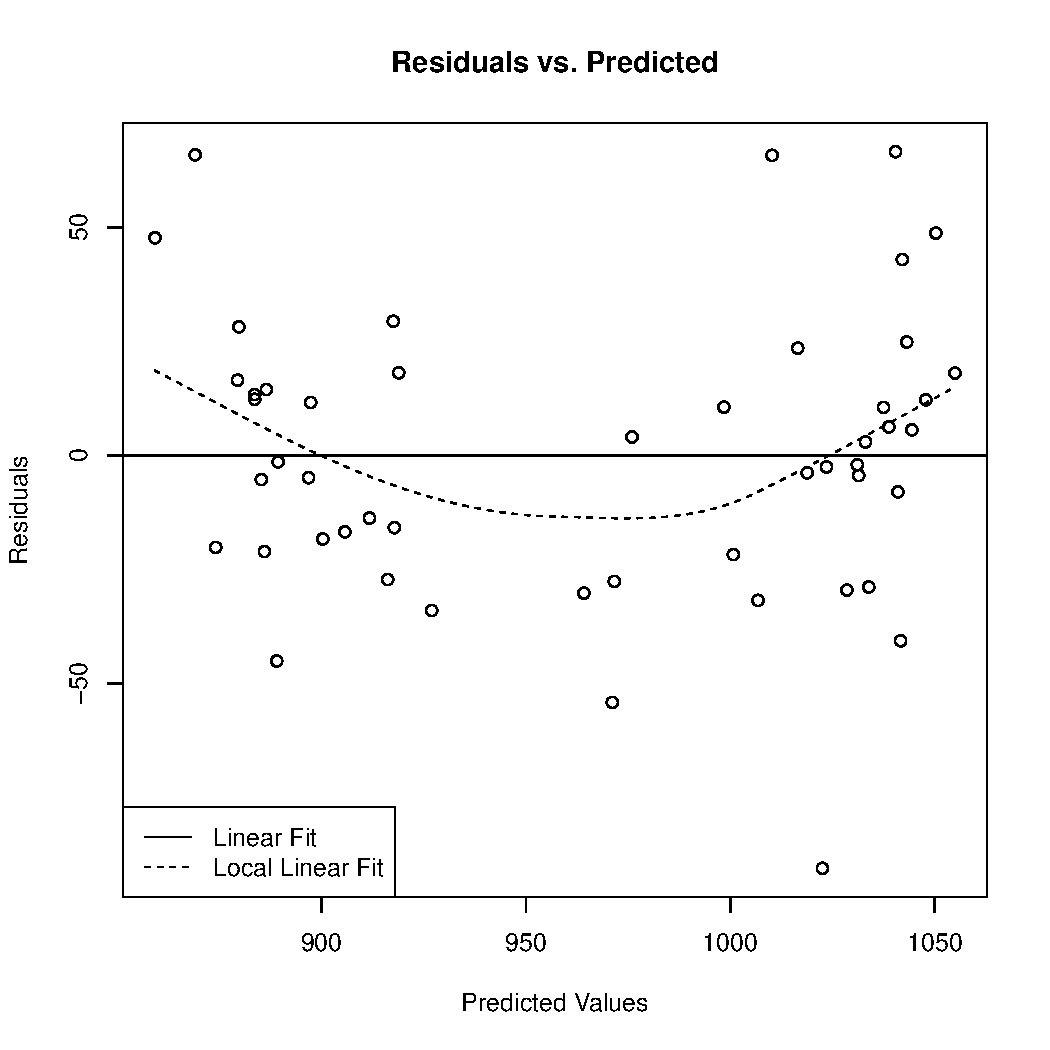
\includegraphics[width=9cm]{hw5_1_f_locfitres} 
                \end{center}
                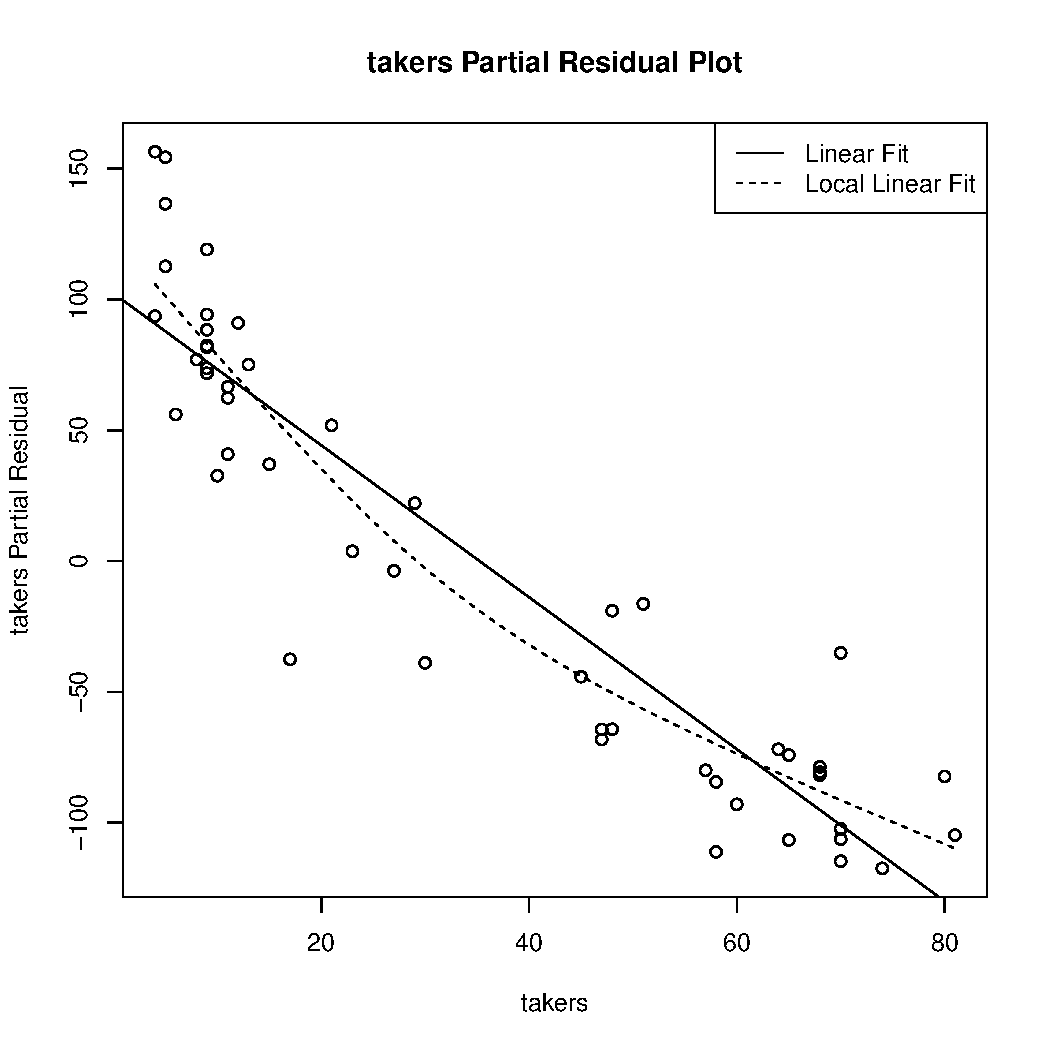
\includegraphics[width=9cm]{hw5_1_f_takers}
                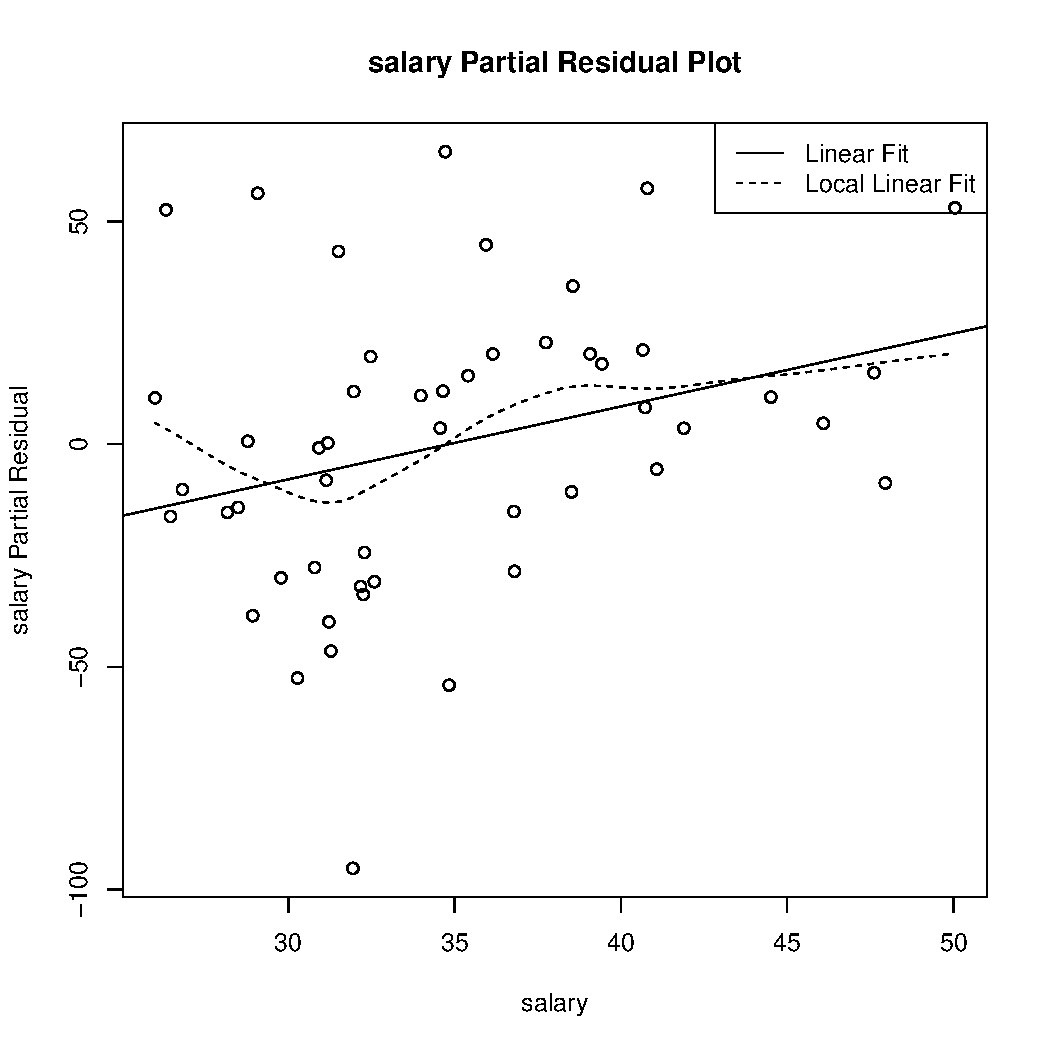
\includegraphics[width=9cm]{hw5_1_f_salary} \\
                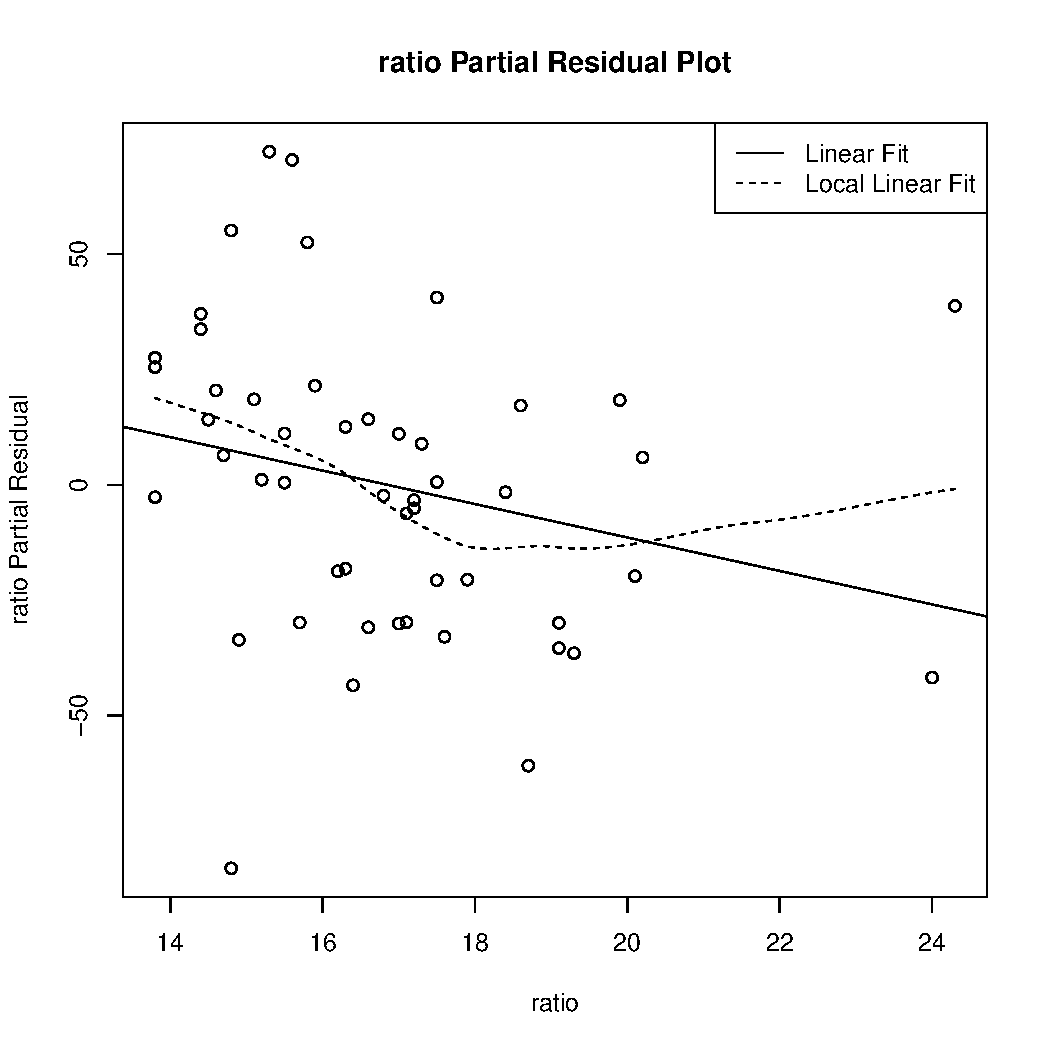
\includegraphics[width=9cm]{hw5_1_f_ratio}  
                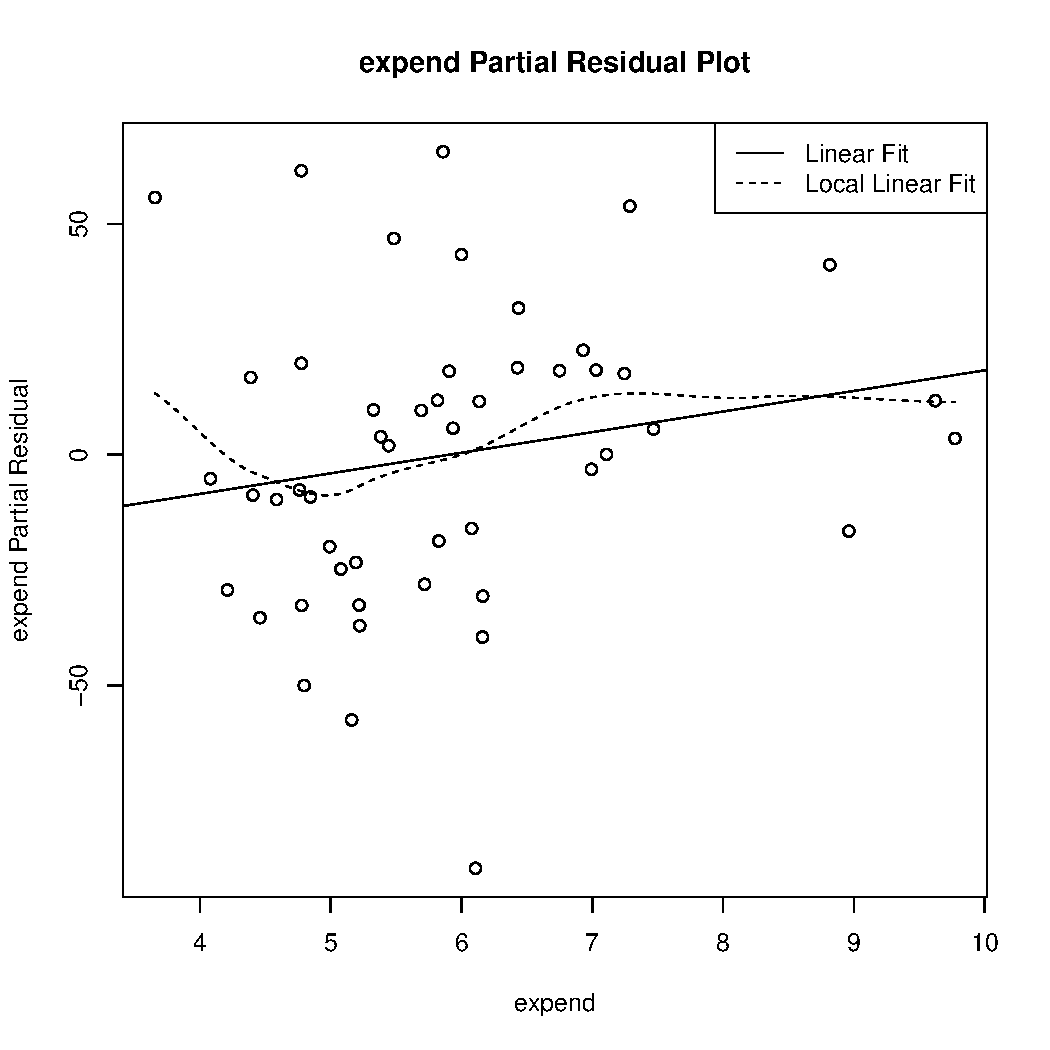
\includegraphics[width=9cm]{hw5_1_f_expend} \\ 
        \end{itemize}
    \item[2.]
        \begin{itemize}
            \item[a)]
                There are only discrete values for waiting, which is in minutes. This indicates that there is some kind of rounding error, where the actual waiting time was rounded to the minute. Since there is no reason to expect that an eruption was more or less likely based on how close the actual time was to a full minute, I am going to assume that the error is uniformly distributed from $-.5$ to $.5$. In other words, I am assuming the time was rounded to the nearest minute. 
                \begin{center}
                    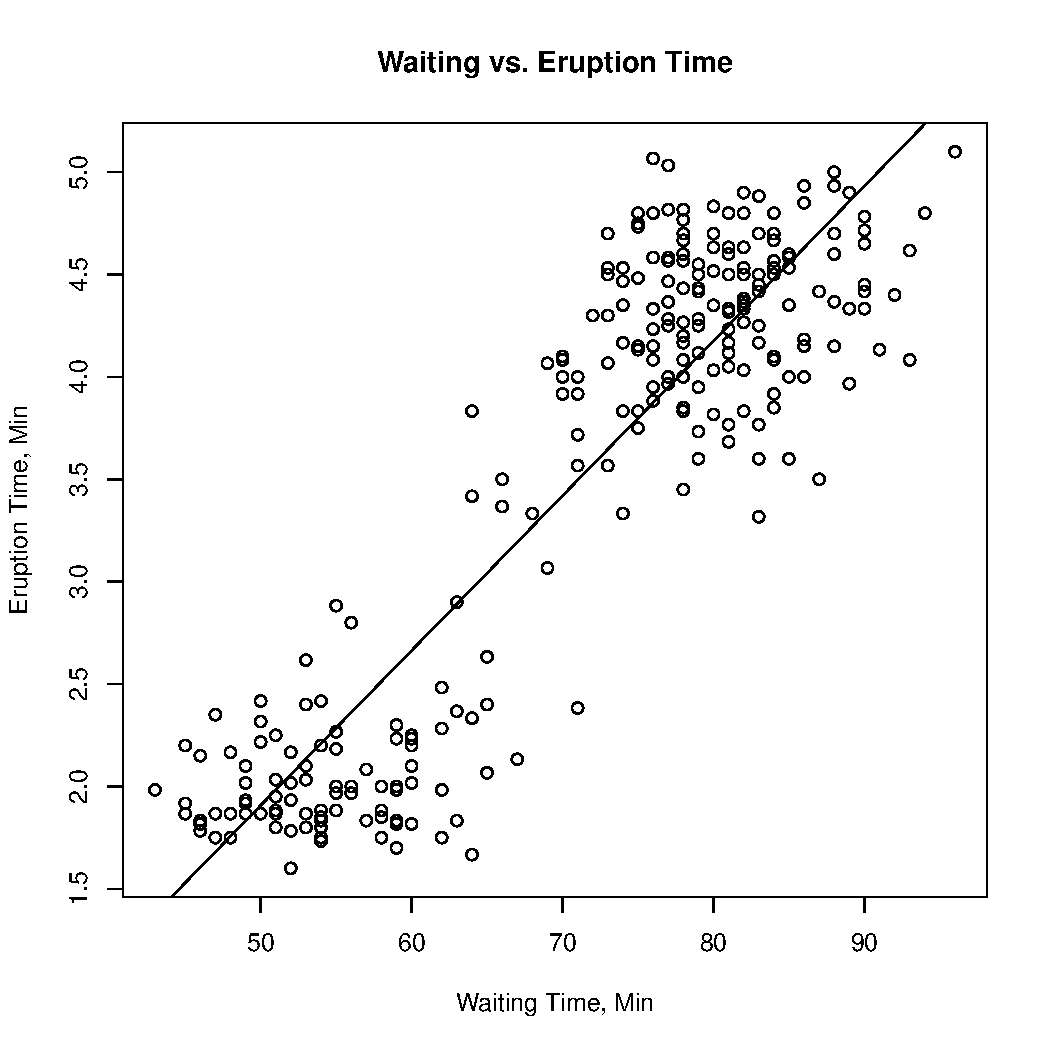
\includegraphics[width=9cm]{hw5_2_a} 
                \end{center}
                The regression I fit can be seen above. There is an intercept of $-1.8740$, and a coefficient on waiting of $.07563$.
            \item[b)]
                If we have a continuous, uniformly distributed error, we can simulate larger continuous uniform errors by summing it with the right discrete uniform random error. Thus, we can simulate a random error that is uniformly distributed on $(-1.5,1.5)$ by randomly choosing from ${-1,0,1}$ and adding it to the original error, an error on $(-2.5,2.5)$ by randomly choosing from ${-2,-1,0,1,2}$ and so on. Taking the mean beta over $1000$ simulations where a particular discrete error was added to the waiting time and the model was fit, we get a distribution that seems to have a linear relationship between variance and $\beta$. Fitting a linear model to it, we can extrapolate to a measurement error level of $0$, giving us a predicted $\beta$ of $.07565$.
                \begin{center}
                    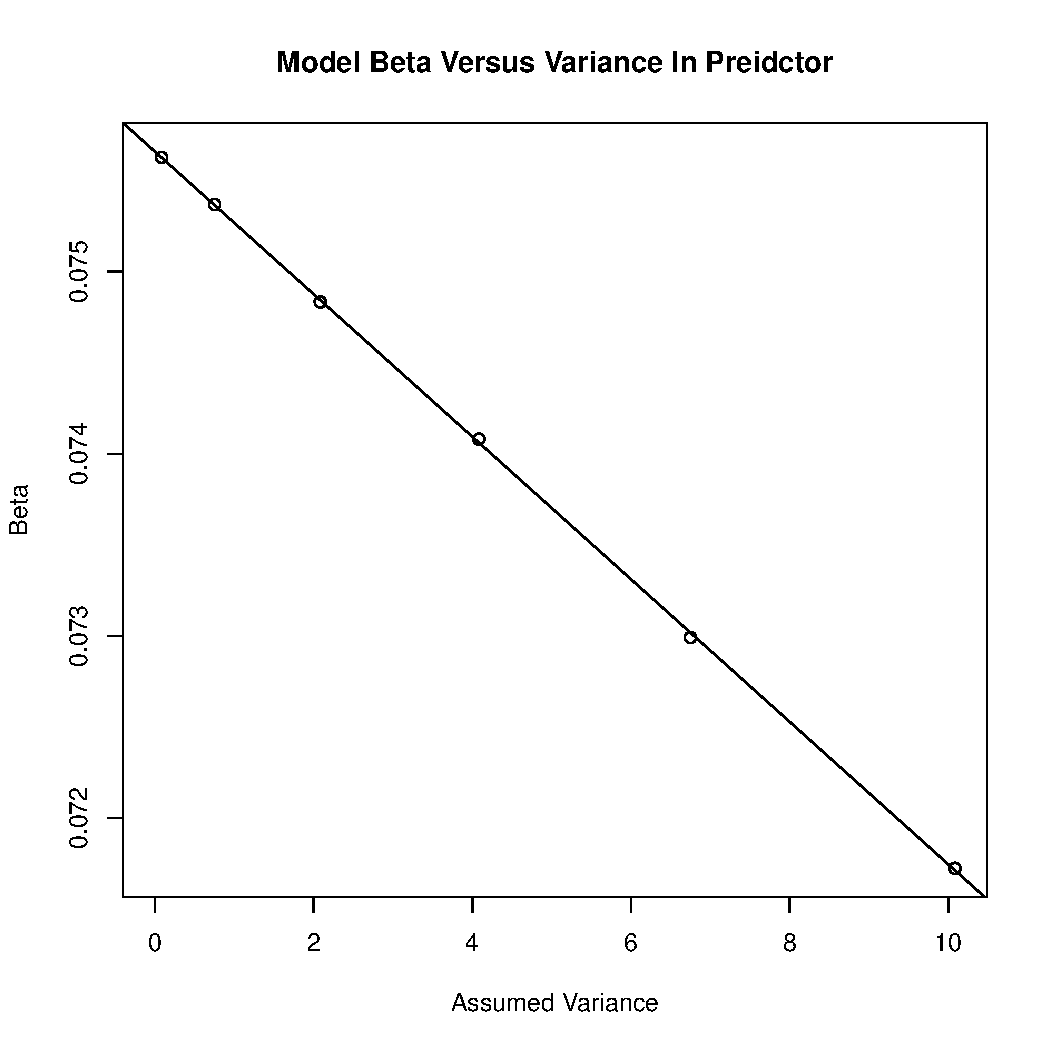
\includegraphics[width=9cm]{hw5_2_b}
                \end{center}
                The above shows the distribution of $\beta$ at different variance levels corresponding to errors uniformly distributed over $(-.5-z,.5+z)$, for $z\in\Z$. These were chosen since, to the best of my knowledge, there is no random variable $X$ such that \(u_{-.5,.5}+X \sim u_{-.5-q,.5+q}\) when $q\not\in\Z$, making these errors hard to simulate.
            \item[c)] If we tried to apply the SIMEX method to variance in the response variable, by running the regression with additional variance added, the expectation of $\beta$ would still be the same irrespective of additional noise, and any fluctuation would be distributed around the original $\beta$. Thus, our extrapolation to $0$ variance would give the same $\beta$. \\
                {\bf Proof:} Let $Y$ be the original set of responses, and $Y^*=Y+e$ for some random variable $e$ with expectation $0$. Thus, \(\E(y^*)=y,\E(\bar y^*) = \bar y\), and \(\E(y^*-\bar y^*) = y -\bar y\). Now, starting with the coefficient on the predictor for a model fit on $Y^*$, $\beta^*$,
                \begin{align*}
                    \beta^* &= r_{xy}\frac{SD_{y^*}}{SD_x} \\
                    \beta^* &= \frac{s_{xy}}{SD_x SD_{y^*}}\frac{SD_{y^*}}{SD_x} \\
                    \beta^* &= \frac{\sum(x_i-\bar x)(y_i^*-\bar y^*)}{(n-1)SD_x^2}\\
                    \E[\beta^*] &= \E\left[\frac{\sum(x_i-\bar x)(y_i^*-\bar y^*)}{(n-1)SD_x^2}\right] \\
                    \E[\beta^*] &= \frac{\sum(x_i-\bar x)(y_i-\bar y)}{(n-1)SD_x^2} \\
                    \E[\beta^*] &= \beta \\
                \end{align*}
                So in the expectation, you would get the same $\beta$ irrespective of the variance level.
            \item[d)]
                \begin{center}
                    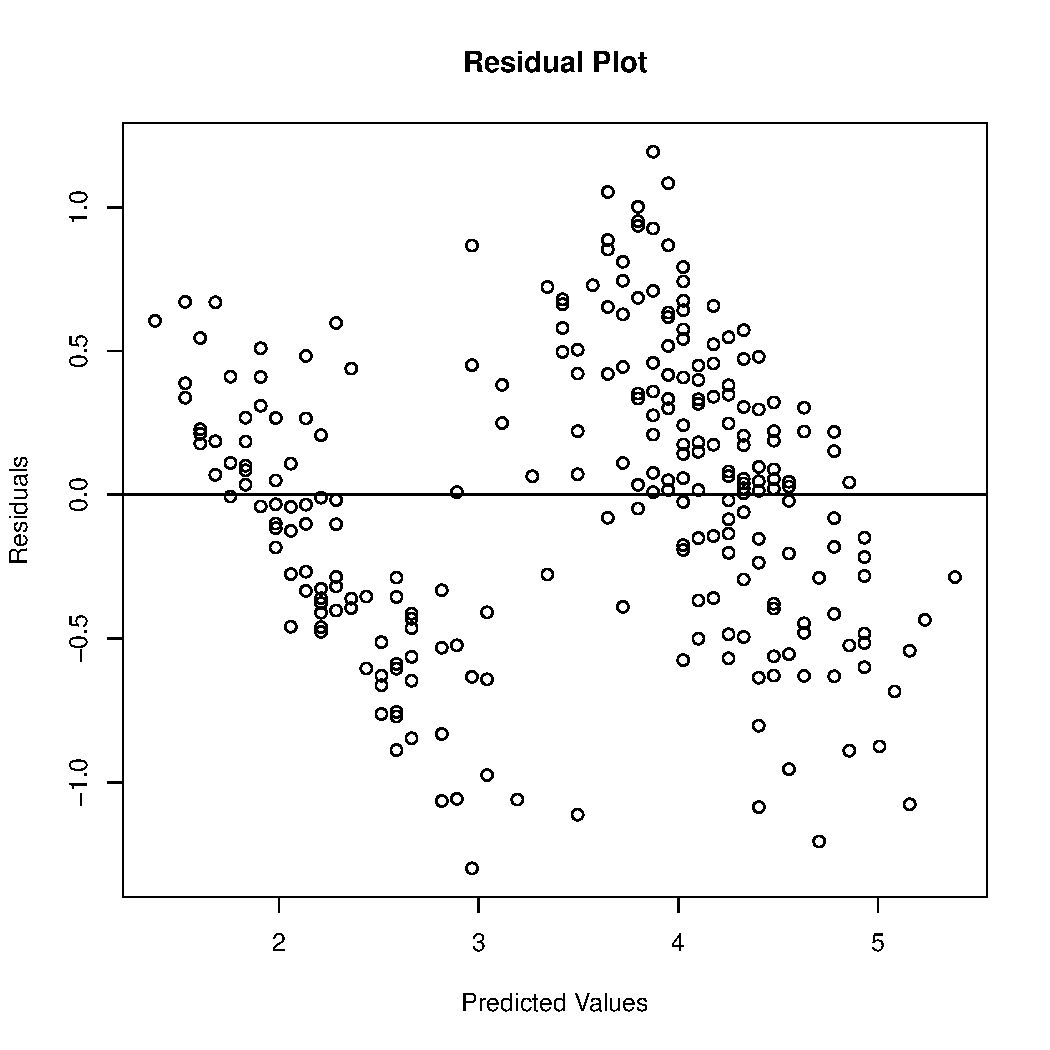
\includegraphics[width=9cm]{hw5_2_d}
                \end{center}
                The residual plot above seems to show that the data really represents two separate regions, for each of which we are systematically underestimating the lower end and overestimating the higher end. The split here corresponds to approximately a waiting time of $68$. This would suggest we really need two different models for waiting times above and below $68$. To test this, I fit a new model which had three new variables.
                \begin{itemize}
                    \item[1-] A binary for whether the waiting time was higher than $68$
                    \item[2-] A variable which was the waiting time if higher than $68$ and otherwise $0$.
                    \item[2-] A variable which was the waiting time if lower than $68$ and otherwise $0$.
                \end{itemize}
                This is essentially two separate models. Since the original model corresponds to a subspace of this model (where the coefficient on the first variable is $0$ and the second two hav equal coefficients), we can compare the two models with a $F$ test: \\
                \begin{table}[ht]
                \centering
                \begin{tabular}{lrrrrrr}
                    \hline
                       & Res.Df & RSS & Df & Sum of Sq & F & Pr($>$F) \\ 
                        \hline
                        1 & 270 & 66.56 &  &  &  &  \\ 
                          2 & 268 & 40.21 & 2 & 26.35 & 87.83 & 0.0000 \\ 
                           \hline
                   \end{tabular}
               \end{table} \\
               Since the p-value is far below $.05$, we can reject the null hypothesis that the original linear model is sufficient, and accept that really two separate models are needed.
        \end{itemize}
    \item[3.]
        \begin{itemize}
            \item[a)]
                Simulating the largest studentized residual on the star data set, I found that there was a larger studetnized residual in the simulation $.974$ of the time. On the savings data set, there was a larger studentized residual $.312$ of the time. I would reject the corresponding point as an outlier at $.05$, since that's the accepted threshold, and in this case would indicate that there is only a $.05$ chance of the point fitting the model so poorly if it indeed came from it.
            \item[b)]
                I found that $.219$ of the simulations of the star data set had a point with as big a Cook Distance. $.408$ of the simulations of the savings data set had a point with as big a Cook Distance. I would not exclude a point automatically at any confidence level of the Cook Statistic, since having a high value is indicative of being influential, but not necessarily a poor fit for the model.
            \item[c)] Both of these conclusions are similar to the analysis from class. With studentized residuals, we checked against the Bonferroni critical value to decide to exclude a point, while with Cook Distance we merely noted high values for further evaluation.
        \end{itemize}
    \item[4.]
        \[ M^{-1} = \left[\begin{array}{cc} H^{-1}+H^{-1}e(f^T-e^TH^{-1}e)^{-1}e^TH^{-1} & -H^{-1}e(f-e^TH^{-1}e)^{-1} \\ -(f^T-e^TH^{-1}e)^{-1}e^TH^{-1} & (f-e^TH^{-1}e)^{-1} \end{array} \right] \]
        {\bf How I Got Here:} First, I assumed that, since $M$ has nice symmetry,
    \[M^{-1} = \left[\begin{array}{cc} A & B \\ B^T & C \end{array}\right] \]
        Since $H$ is positive definite, it has an inverse. Since it is symmetric, the inverse is as well. Since \(MM^{-1}=I\), we get that
        \[HA+eB=I, \, HB+eC=0, \, e^TA+fB^T=0, \, e^TB+fC=I\]
        From the second equation, using $H^{-1}$, we get \(B=-H^{-1}eC\). Plugging this into the fourth equation, we get that \((f-e^TH^{-1}e)C=I\). Since we can repeat this process for \(M^{-1}M=I\) and get \(C(f-e^TH^{-1}e)=I\), we can conclude that $C$ is invertible with \(C=(f-e^TH^{-1}e)^{-1}\). Plugging the first two results into the first equation, we get
        \[HA-e(f-e^TH^{-1}e)^{-1}e^TH^{-1}=I\]
        so
        \[A=H^{-1} + H^{-1}e(f-e^TH^{-1}e)^{-1}e^TH^{-1}\]
        Plugging everything in and multiplying $MM^{-1}$, I get the desired result, so my initial assumption appears to be correct.
    \item[5)]
        Since 
        \[r_{u,v}=\frac{\langle u - \bar u, v -\bar v\rangle}{\|u-\bar u\|\|v-\bar v\|} \]
        if \(r_{x,y}=\pm 1\) and \(\bar v = \bar u = 0\), we get that
        \[\vert\langle u, v\rangle\vert = \|u\|\|v\| \]
        By Cauchy-Schwarz, this implies that \(u\) and \(v\) are linearly dependent. Accordingly, the design matrix, which is \( [\begin{array}{cc}u & v\end{array}]\), will only have one linearly independent column, and will thus have a rank of 1.
        \smallskip
        To get the variance of the estimators, we need to get the covariance matrix of the coefficient vector:
        \begin{align*}
            \cov\left[\begin{array}{c}\hat a \\ \hat b \end{array}\right] &= \sigma^2\left([\begin{array}{cc}u & v\end{array}]^T[\begin{array}{cc}u & v\end{array}]\right)^{-1} \\
            \left[\begin{array}{cc} \var(\hat a) & \cov(\hat a,\hat b) \\ \cov(\hat a,\hat b) & \var(\hat b) \end{array} \right] &= \left[\begin{array}{cc} \|u\|^2 & \langle u, v \rangle \\ \langle u, v \rangle & \|v\|^2 \end{array} \right]^{-1} \\
            \left[\begin{array}{cc} \var(\hat a) & \cov(\hat a,\hat b) \\ \cov(\hat a,\hat b) & \var(\hat b) \end{array} \right] &= \frac{1}{\|u\|^2\|v\|^2-\langle u, v \rangle^2} \left[\begin{array}{cc} \|u\|^2 & -\langle u, v \rangle \\ -\langle u, v \rangle & \|v\|^2 \end{array} \right] \\
            \left[\begin{array}{cc} \var(\hat a) & \cov(\hat a,\hat b) \\ \cov(\hat a,\hat b) & \var(\hat b) \end{array} \right] &= \frac{1}{\|u\|^2\|v\|^2(1-r^2)} \left[\begin{array}{cc} \|u\|^2 & - r\|u\|\|v\| \\ -r\|u\|\|v\| & \|v\|^2 \end{array} \right]
        \end{align*}
        Pulling what we need out of this, we get that \(\var(\hat a) = \frac{\|u\|^2}{\|u\|^2\|v\|^2(1-r^2)}\), \(\var(\hat b) = \frac{\|v\|^2}{\|u\|^2\|v\|^2(1-r^2)}\),
        \[\var(\hat a + \hat b) = \var(\hat a) + \var(\hat b) + 2\cov(\hat a,\hat b) = \frac{\|u\|^2 + \|v\|^2 - 2r\|u\|\|v\| }{\|u\|^2\|v\|^2(1-r^2)}\]
        and
        \[\var(\hat a - \hat b) = \var(\hat a) + \var(\hat b) - 2\cov(\hat a,\hat b) = \frac{\|u\|^2 + \|v\|^2 + 2r\|u\|\|v\| }{\|u\|^2\|v\|^2(1-r^2)}\]
        So, when $r=-.99$, we are going to see $\var(\hat a + \hat b)$ be large, since its numerator is large and its denominator is small (compared to a less negative $r$). $\var(\hat a)$ and $\var(\hat b)$ are going to have a small denominator, so they will also be large. Only $\var(\hat a - \hat b)$, with a numerator that shrinks as $r$ decreases will be relatively small. This means that \(\hat a - \hat b\) will be the easiest to estimate, while the others will be relatively harder.  
    \item[6)]
        \begin{itemize}
            \item[a)]
                I've calculated the condition number, which is, for each eigenvalue $\lambda$, \(\sqrt{\frac{\lambda}{\lambda_{min>0}}}\), below. The largest condition number is an astronomical $5751.22$, which is way higher than the $30$ which is considered large. That we have several other that are also large indicates we have several variables which are independently extremely close to linear combinations of other variables. All in all this dictates a lot of multicollinearity. \\
                \begin{table}[ht]
                    \centering
                    \begin{tabular}{rrrrrrr}
                          \hline
                           & 1 & 2 & 3 & 4 & 5 & 6 \\ 
                            \hline
                            1 & 5751.22 & 322.11 & 228.65 & 94.62 & 3.49 & 1.00 \\ 
                               \hline
                           \end{tabular}
                       \end{table}
            \item[b)] 
                I have calculated the pairwise collinearity below. We see a number of variables which have pairwise collinearities very close to one, such as between Year and GNP or Year and Population. This supports the notion from part a) that their is a ton of collinearity, showing several variables are pairwise collinear, though not addressing any multicollinearity. \\
                \begin{table}[ht]
                    \centering
                    \begin{tabular}{rrrrrrr}
                          \hline
                           & GNP.deflator & GNP & Unemployed & Armed.Forces & Population & Year \\ 
                            \hline
                            GNP.deflator & 1.00 & 0.99 & 0.62 & 0.47 & 0.98 & 0.99 \\ 
                              GNP & 0.99 & 1.00 & 0.60 & 0.45 & 0.99 & 0.99 \\ 
                              Unemployed & 0.62 & 0.60 & 1.00 & -0.18 & 0.69 & 0.67 \\ 
                              Armed.Forces & 0.47 & 0.45 & -0.18 & 1.00 & 0.36 & 0.42 \\ 
                              Population & 0.98 & 0.99 & 0.69 & 0.36 & 1.00 & 0.99 \\ 
                              Year & 0.99 & 0.99 & 0.67 & 0.42 & 0.99 & 1.00 \\ 
                               \hline
                           \end{tabular}
                       \end{table}
            \item[c)]
                The variance inflation factors below are calculated as \(\frac{1}{1-R_j^2}\), where \(R_j^2\) is the $R^2$ of a regression predicting one predictor variable using all the other predictor variables. That these are so high speak to the collinearity we've already observed. More specifically though, high variance inflation factors dictate that the estimate of the coefficient will have high variance. Thus, our estimates of the coefficients for GNP, Year, Population, among others, are going to be very noisy. \\
                \begin{table}[ht]
                    \centering
                    \begin{tabular}{rrrrrrr}
                          \hline
                           & GNP.deflator & GNP & Unemployed & Armed.Forces & Population & Year \\ 
                            \hline
                            1 & 135.53 & 1788.51 & 33.62 & 3.59 & 399.15 & 758.98 \\ 
                               \hline
                           \end{tabular}
                       \end{table}
        \end{itemize}
\end{itemize}
\end{document}
